%\begin{sidewaysfigure}
%  \begin{center}
%  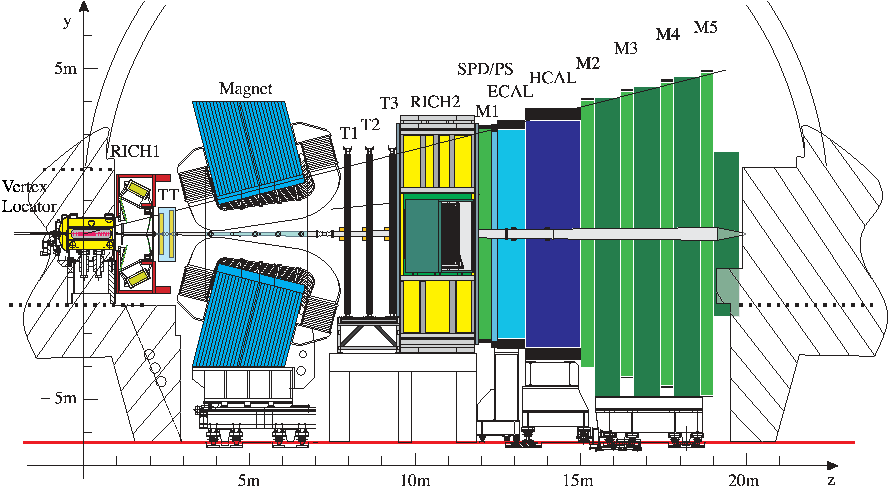
\includegraphics[width=0.8\textheight]{lhcb-detector-cross-section}
%  \caption[Cross-section view of \LHCb, cut in the non-bending $y$--$z$ plane]%
%    {Cross-section view of \LHCb, cut in the non-bending $y$--$z$ plane.}
%  \label{fig:LHCbCrossSection}
%  \end{center}
%\end{sidewaysfigure}



\chapter{ND280 ECal event reconstruction and software}
\label{chap:ND280Software}
Lots of software stuff

\section{Real data processing}
\label{sec:datachain}
Process the data.  MAY NOT INCLUDE THIS

\section{Monte Carlo event simulation}
\label{sec:MCchain}
Process the MC

\subsection{Neutrino flux prediction}
\label{subsec:NeutrinoFluxPrediction}
I guess the flux is quite bit

\subsection{Neutrino interaction simulation}
\label{subsec:NeutrinoInteractionSimulation}
NEEEEEUT

\subsection{ND280 detector simulation}
\label{subsec:ND280DetectorSimulation}
nd280mc is really good for this

\subsection{Detector response simulation}
\label{subsec:DetectorResponseSimulation}
Is elecSim there?

\subsection{Detector calibration}
\label{subsec:DetectorCalibration}
oaCalib calibrates

\subsection{Event reconstruction}
\label{subsec:EventReconstruction}
oaRecon yo!

\section{ECal event reconstruction}
\label{sec:ECalEventReconstruction}
All about ecalRecon

\subsection{Hit preparation}
\label{subsec:ECalHitPerparation}
Hit prep

\subsection{Basic clustering}
\label{subsec:ECalBasicClustering}
Baaasic

\subsection{Cluster combination}
\label{subsec:ECalCombineClusters}
Combine dem clusters

\subsection{Cluster expansion}
\label{subsec:ECalExpandClusters}
Expand dem clusters

\subsection{3D cluster formation}
\label{subsec:ECal3DMatching}
Match the clusters

\subsection{3D hit reconstruction}
\label{subsec:ECal3DHitReconstruction}
Least square those fits

\subsection{Energy reconstruction}
\label{subsec:ECalEnergyReconstruction}
blah

\subsection{Event classification}
\label{subsec:ECalParticleIdentification}
Track or shower?
